\section{Arquitectura de Redundancia Propuesta}

En esta sección, se presenta la arquitectura implementada para la tolerancia a fallas de hardware. Como se mostró en la sección anterior, \textit{The Byzantine Generals Problem} sienta las bases para la tolerancia a fallas arbitrarias de hardware. A través de una serie de intercambios de mensajes entre los nodos de la red, estos pueden llegar a un consenso, para tomar la misma decisión. Además, se mostró que para poder tolerar una falla arbitraria, se requiere por lo menos de 4 nodos interconectados.

Luego de presentar el problema, se hizo una comparación entre los generales leales y las computadoras de vuelo sin fallas y entre los generales traidores y las computadoras con fallas. Una de las cuestiones que no se mencionó, es el hecho de que las computadoras de vuelo constituyen sistemas de tiempo real. Esto es debido a que deben realizar tareas que requieren determinismo temporal. Por ejemplo, cálculo de la ley de control, estimación de la pose, etc... En el problema original, los generales pueden enviar sus mensajes a sus pares en cualquier momento y en cualquier orden.

Otro de los puntos que caracterizan al problema original, es el hecho de que la comunicación entre los generales es 1 a 1. Debido a esto, los generales traidores pueden entregar información confusa a sus pares para tratar de romper el consenso. Esto es lo que vuelve complejo al problema \cite{lamport2019byzantine} y costosa a su solución \cite{roth2021not}.

En esta sección se muestra que, si el sistema tiene ciertas características, en particular ser un sistema de tiempo real y contar con un bus común a los nodos para las comunicaciones, luego el problema del consenso se simplifica mucho.

\subsection{Simplificación del Problema de Tolerancia a Fallas Arbitrarias de Hardware}

En sistemas de tiempo real para aplicaciones \textit{safety-critical}, es común encontrar sistemas distribuidos con comunicación a través de un bus. Por ejemplo en los automóviles, los nodos que se encuentran repartidos por todo el vehículo se comunican a través de redes como CAN\cite{specification1991bosch} o FlexRay\cite{nxpAN12233}. Todos los nodos de la red se encuentran conectados al mismo bus de comunicación, por lo que cuando un nodo envía un mensaje a través del bus, todos los demás nodos reciben el mismo mensaje.

\begin{figure}[H]
    \centering
    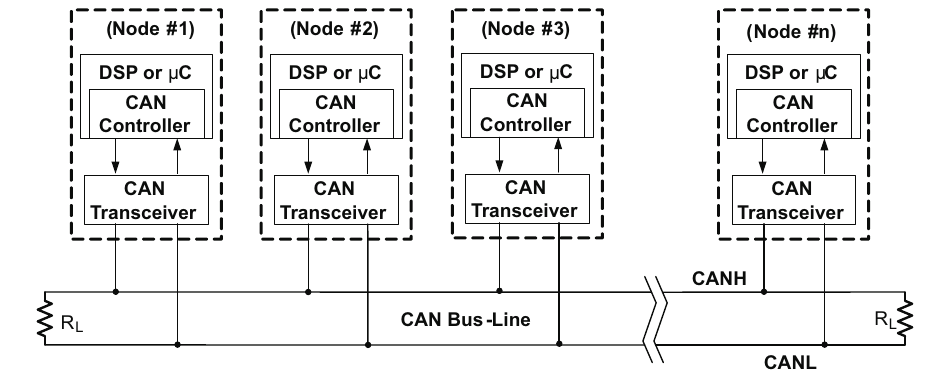
\includegraphics[width=\textwidth]{img/red_CAN.png}
    \caption{Todos los nodos se encuentran conectados al mismo bus de comunicaciones. En el caso del bus CAN, se compone de dos cables, CAN-H y CAN-L, terminados en sus extremos por resistencias de adaptación. La imagen se extrajo de \cite{texasSLOA101B}.}
    \label{fig:red_CAN}
\end{figure}

Esto presenta una diferencia respecto de lo planteado en \textit{The Byzantine Generals Problem}, ya que la existencia de un bus común a todos los nodos automáticamente elimina la posibilidad de que uno de los miembros de la red pueda enviar información diferente a sus pares. Puede compararse la figura \ref{fig:byzantine_bus_1} con la figura \ref{fig:Byzantine_Generals_Problem_5}.

\begin{figure}[H]
    \centering
    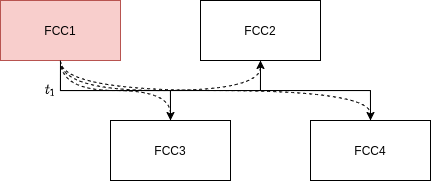
\includegraphics[width=0.6\textwidth]{img/byzantine_bus_1.png}
    \caption{En este caso, la conexión tipo bus no permite el envío de información diferente a los demás miembros. La FCC1 envía el valor $t_1$ y todos sus pares reciben el mismo valor.}
    \label{fig:byzantine_bus_1}    
\end{figure}

Como contrapartida, debido a que los nodos comparten canal de comunicación, estos deben tomar turnos para enviar la información a sus pares. De otra forma, habría una colisión en el bus y la información nunca llegaría a su destino. Sumado a esto, el bus se convierte en un punto singular de falla, ya que es posible que un problema en el bus deje a los nodos incomunicados.

{\Large \textbf{{\color{red} ACÁ AGREGAR EJEMPLOS DE USO DE DOBLE BUS. POR EJEMPLO LOS AUTOS CON DOBLE CAN O DOBLE FLEX RAY, EL PAPER QUE USA DOBLE TIME TRIGGERED BUS, ETC}}}

\subsubsection{Consenso}

Al igual que como se hizo en la sección \ref{sec:consenso_TMR}, se analiza el problema del consenso para la arquitectura propuesta en esta sección. El ejemplo que se presentó anteriormente fue el necesario para lograr una sincronización entre las FCCs y se mostró que el enviar información distinta a cada computadora de vuelo, puede romper el sincronismo muy fácilmente.

Para el caso en el que se utiliza un bus de comunicación, como se mencionó, las FCCs deben tomar turnos para utilizar el medio físico. En las próximas secciones se explicará cómo se puede lograr esto, aquí se asume que las FCCs respetan sus turnos para utilizar el medio físico compartido. En la figura \ref{fig:byzantine_bus_2}, la FCC1 accede al medio y envía su valor de \textit{timestamp}. Las demás FCCs reciben el mismo valor, por estar conectadas al mismo bus de comunicación. Luego, las FCC2 y 3 repiten esto mismo. En la figura \ref{fig:byzantine_bus_3} se muestra que todas tienen la misma información respecto de sus pares. Luego por ejemplo, si calculan un promedio, llegarán al mismo resultado y se sincronizarán correctamente.

\begin{figure}[H]
    \centering
    \begin{subfigure}[b]{0.34\textwidth}
        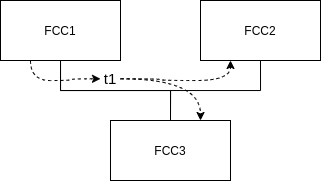
\includegraphics[width=\textwidth]{img/byzantine_bus_2.png}
        \caption{La FCC1 envía su \textit{timestamp} hacia las demás.}
        \label{fig:byzantine_bus_2}
    \end{subfigure}\hfill
    \begin{subfigure}[b]{0.49\textwidth}
        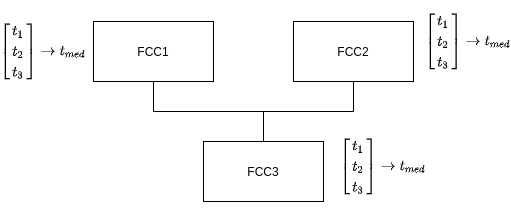
\includegraphics[width=\textwidth]{img/byzantine_bus_3.png}
        \caption{Luego de finalizar los intercambios, todas las FCCs llegan al mismo resultado de \textit{timestamp} para sincronizarse.}
        \label{fig:byzantine_bus_3}
    \end{subfigure}
    \caption{Debido a la existencia del bus, las FCCs no pueden mentir acerca de su \textit{timestamp}. Luego, todas llegan a un consenso de manera casi trivial.}
    \label{}
\end{figure}

A partir de este análisis, se puede ver que para el caso de un sistema de tiempo real con un único bus de comunicaciones, el problema del consenso es mucho más sencillo que lo que se muestra en \textit{The Byzantine Generals Problem}. De todas maneras, lo que se presenta aquí es un primer análisis, ya que se ha asumido que no hay colisiones en el bus y que los nodos se encuentran sincronizados.

\subsubsection{Sincronismo de los nodos}

En la sección \ref{sec:sincronismo_TMR} se mencionó la necesidad del sincronismo entre los nodos y que esta se logra a partir de un intercambio de mensajes. Para la arquitectura propuesta, ese intercambio de mensajes se hace a través del mismo bus. Debido a que el medio es compartido, los nodos de la red deben tomar turnos para acceder al medio, de manera de que todos puedan enviar sus respectivos mensajes.

Típicamente, una FCC ejecuta las mismas tareas relacionadas al control del vehículo, de manera periódica \cite{hiergeist2018implementation}:

\begin{enumerate}
    \item Lectura de los sensores.
    \item Cálculo de la ley de control.
    \item Aplicación del resultado a los actuadores.
\end{enumerate}

Debido a que se trata de un sistema de tiempo real, cada una de las FCCs debe realizar estas tareas en un período de tiempo dado. En la figura \ref{fig:task_scheduling_1} se muestra un gráfico con la secuencia de ejecución periódica de las tareas.

\begin{figure}[H]
    \centering
    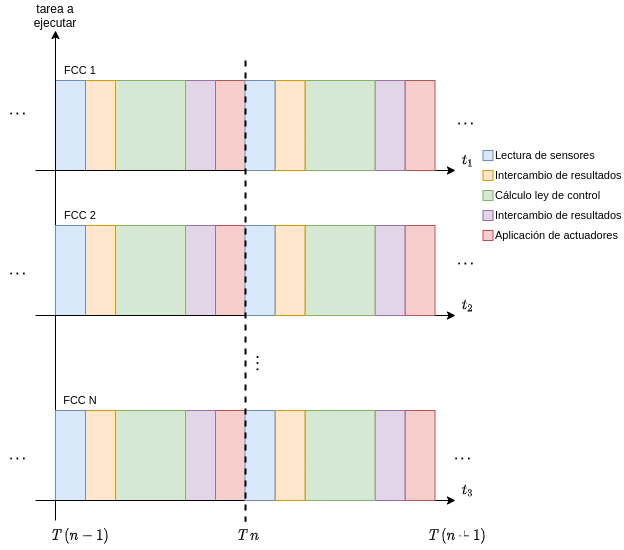
\includegraphics[width=0.7\textwidth]{img/task_scheduling_1.png}
    \caption{El eje horizontal representa el paso del tiempo. Las barras de colores representan el tiempo dedicado a ejecutar cada tarea, como la lectura de sensores, cálculo de la ley de control, etc., de forma periódica. En la imagen se puede ver que las FCC 1, FCC 2, ..., FCC N se encuentran sincronizadas ya que realizan las tareas al mismo tiempo. }
    \label{fig:task_scheduling_1}
\end{figure}

En un sistema con redundancias, como ya se mencionó, cada una de las FCCs realiza las mismas tareas. Además, estas intercambiarán resultados relacionados a mediciones de sensores y a valores de actuación para los motores con sus pares, justamente para enmascarar y tolerar las fallas. A partir de esto, se desprende que el intercambio de mensajes también corresponde a tareas que deben ejecutarse periódicamente y en un determinado período de tiempo acotado.

Cada una de las computadoras de vuelo incluye un clock interno, el cual utiliza como base para cumplir con los tiempos de ejecución. Cuando se habla del sincronismo entre los nodos de la red, lo que se busca es que las ejecuciones de las N computadoras se encuentren coordinadas. Por ejemplo, en la figura \ref{fig:task_scheduling_2} se muestra un caso para dos computadoras de vuelo cuya ejecución se encuentra desfasada. Es fácil ver que este sistema nunca podrá cumplir con el objetivo de controlar el vuelo del UAV.

\begin{figure}[H]
    \centering
    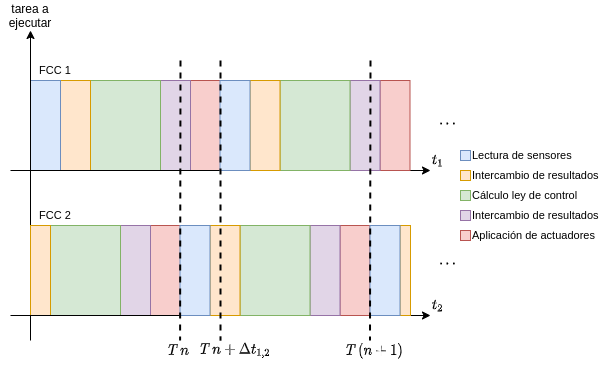
\includegraphics[width=0.7\textwidth]{img/task_scheduling_2.png}
    \caption{Se muestra un ejemplo para dos FCCs. A diferencia de la figura \ref{fig:task_scheduling_1}, las FCC 1 y la FCC 2 se encuentran desincronizadas.}
    \label{fig:task_scheduling_2}
\end{figure}


En la figura, se muestra que cuando la FCC 2 termina de enviar la señal de control a los actuadores (instante $T_n$), la FCC 1 se encuentra intercambiando resultados con la FCC 2. Debido a que la FCC 2 ya pasó dicha tarea, la FCC 1 no recibirá ningún valor de su par y asumirá erróneamente, que la FCC 2 se encuentra en un estado con alguna falla, ya que no responde. Si bien este ejemplo es muy simple, muestra la necesidad de la sincronización entre nodos de la red, siendo el motivo principal, el hecho de que el sistema es de tiempo real.

\subsection{Arquitectura Utilizada: \textit{The Time-Triggered Architecture}}